\chapter[Processo de Engenharia de Requisitos]{Processo de Engenharia de Requisitos}\label{cap4}

Esse processo foi desenhado utilizando ferramenta ``\textit{BIZAGI modeler}''. Houveram 5 evoluções,
presentes no apêndice \ref{apendice:evolution}, a partir do primeiro esboço até chegar a versão apresentada na imagem \ref{fig:processo}. Para criação das atividades do processo
a equipe criou um \textit{framework} de mapeamento entre Abordagens de Engenharia de \textit{Software}, Modelos de Maturidade e Atividades Fundamentiais da Engenharia de Requisitos. Este framework se encontra
no apêndice \ref{apendice:mapeamento} justificando a presença de cada atividade.

Como foi descrito no capítulo \ref{cap3} o processo criado foi estruturado baseando-se no
SAFe mantendo os três níveis estruturais do \textit{framework}, portfólio, programa e time
que estão detalhados na sessão \ref{safe}.

A manutenção da rastreabilidade dos requisitos, tem papel fundamental para a criação deste processo,
entretando no processo SAFe não há a definição plena da manutenbilidade da rastreabilidade entre os
vários níveis. Portanto há a necessidade de criação de uma adaptação, para isso utiliza-se de
outro processo base, o RUP.

É fundamental destacar que o problema da escolha de um abordagem não esta em considerar
a mutabilidade dos requisitos e sim em como tratar essas mudanças que são inevitáveis.
Pensando nisso foram adicionadas atividades de gerência de mudanças baseadas no RUP,
para sanar um possível risco na comunicação e gerência do projeto devido a não experiência
de trabalho entre os membros do grupo. Esse processo ocorre de forma eventual e paralela
e será detalhado na sessão \ref{sec:gerencia}.

\begin{figure}[H]
    \centering
	\includegraphics[keepaspectratio=true,scale=0.5]{figuras/Processo_05.eps}
    \caption{Visão geral do processo desenvolvido para o projeto.}
    \label{fig:processo}
\end{figure}

\section{Scaled Agile Framework}\label{safe}

Nessa sessão serão descritos os níveis que compoem o SAFe(portfólio, Programa e Time).
Sendo mostrado o objetivo cada nível como também as atividades que a compoem.

\section{portfólio}

No processo criado nesse trabalho, esse nível tem como objetivo levantar e estabelecer
uma abstração de alto nível dos requisitos do negócio. Esse levantamento ocorrerá
por meio da efetuação das atividades Entender Contexto do Cliente e Levantar Épicos
e Revisar e Analisar. As técnicas utilizadas para a execução de cada atividade serão
a análise documental, \textit{Workshop} e Brainstorms.

\subsection{Processo}

\begin{figure}[H]
    \centering
  \includegraphics[keepaspectratio=true,scale=0.5]{figuras/portifa.eps}
    \caption{Visão geral do nível de portfólio.}
    \label{fig:portifa}
\end{figure}

\subsection{Papéis}

\textbf{Gerente de Portfólio}: Possui a mais alto nível de decisão do processo, buscam compreender
a estratégia da empresa, tecnologia e restrições. No nosso contexto ele terá também
a função de Dono do Épico, que é responsável pela condução dos épicos para identificação
através da análise do processo e do sistema Kanban. Quando aceito para implementação,
trabalha com a equipe de desenvolvimento e de gestão de produtos para iniciar as atividades
de desenvolvimento necessárias para contemplar o épico.

\subsection{Artefatos}



\begin{description}
  \item[A - Processo do cliente:]
  Artefato de entrada que será fornecido pelo cliente ao Gerente de portfólio.
  Contém o processo otimizado, da organização do cliente, modelado na notação BPMN.\cite{BPMN}
  \item [B - Contexto do cliente]
  Artefato fornecido pelo cliente, que descreve resumidamente o contexto do problema
  a ser solucionado e uma síntese do motivo da contratação para o desenvolvimento de software.
  \item [C - Tema de investimento: ]
  Representa os objetivos do financiamento da solução, área que irá atuar e valores da empresa.
  É representado por uma pequena proposição com uma breve descrição. É o requisito de
  mais alto nível no processo. Compoem o portifolio backlog.\cite{themes}
  \item [D - Lista de Épicos:]
  Os épicos representam uma iniciativa de negócio, pode ser algo que gere alto valor
  para o cliente ou alto valor para o desenvolvimento de software, como inovações de arquitetura.
  É um requisito ainda de alto nível e deve ser sempre coletado, analisado e refinado.
  Possui três níveis de dimensão
    \begin{enumerate}
      \item \textbf{Tempo: } A implementação pode levar muitas iterações e releases.
      \item \textbf{Escopo: } Afeta vários níveis no projeto, por ser alto nível a mudança
      de um épico pode ocasionar um grande impacto e custar muito para a organização.
      \item \textbf{Negócio: } Afeta vários departamentos na área de negócios, representa
      a entrega de valor direta para o cliente no portfólio.
    \end{enumerate}
  A lista de épicos é o resultado de um brainstorm de possíveis épicos para serem entregues,
  que passarão depois por uma atividade para filtrar e analisar a consistensia dos mesmos.
  \item [E - \textit{Backlog} do Portfólio]
  \textit{Backlog} de portfólio: É uma pilha que contem os épicos detalhados e organizados
  por ordem de prioridade de implementação. É feito uma estimativa em pontuações
  que representam a complexidade do épico. Para fazer essa estimativa o épico deve
  ser detalhado para facilitar a identificação de possível divisão desse épico em
  outros épicos, e a análise da consistência do mesmo.\cite{epics}

  Para estimar o valor do épico, pode ser utilizado o template no apêndice \ref{apendice:templates}
\end{description}

\subsection{Atividades}

  \begin{table}[H]
    \centering
      \begin{tabular}{| m{5em} | m{10cm} |}
        \hline
        ID       & 01   \\ \hline
        Nome     & Entender Contexto do Cliente   \\ \hline
        Objetivo & Serão realizadas reuniões entre o cliente e o gerente de portfólio para um primeiro contato com o objetivo de entender e esclarecer o contexto do problema. \\ \hline
        Entradas & Processo do Cliente, Contexto do Cliente.   \\ \hline
        Saídas   & Tema de Investimento. \\ \hline
        Papel Responsável   & Gerente de Portfólio. \\ \hline
      \end{tabular}
      \caption{Atividade: Entender Contexto do Cliente }
      \label{tabela:atividade1}
  \end{table}

  \begin{table}[H]
    \centering
      \begin{tabular}{| m{5em} | m{10cm} |}
        \hline
        ID       & 02   \\ \hline
        Nome     & Levantar Épicos   \\ \hline
        Objetivo & \textit{Brainstorm} de ideias relacionadas ao tema de investimento e escrita de épicos. \\ \hline
        Entradas & Tema de Investimento   \\ \hline
        Saídas   & Lista de Épicos \\ \hline
        Papel Responsável   & Gerente de Portfólio. \\ \hline
      \end{tabular}
      \caption{Atividade: Levantar Épicos}
      \label{tabela:atividade2}
  \end{table}

  \begin{table}[H]
    \centering
      \begin{tabular}{| m{5em} | m{10cm} |}
        \hline
        ID       & 03   \\ \hline
        Nome     & Selecionar e Detalhar Épicos   \\ \hline
        Objetivo & Os épicos levantados são filtrados, pois podem surgir épicos não alinhasdos com o tema de investimentos. Serão também detalhados, analisados e revisados. Algumas \textit{Features}  podem surgir e irão compor a versão inicial do \textit{Backlog} do Programa. Só é possível a saída da atividade após a aprovação do Gerente. Aqui acontece o primeiro ponto de verificaçã o de mudanças e processo. \\ \hline
        Entradas & Lista de Épicos   \\ \hline
        Saídas   & \textit{Backlog} do Programa, \textit{Backlog} do portfólio(Atualizado). \\ \hline
        Papel Responsável   & Gerente de Portfólio. \\ \hline
      \end{tabular}
      \caption{Atividade: Selecionar e Detalhar Épicos}
      \label{tabela:atividade3}
  \end{table}

  \section{Programa}

  Nesse nível do processo, foram definidas as atividades Levantas Requistos não funcionais,
  Selecionar Épicos para a Iteração, Levantar \textit{Features} , Levantar Histórias de Usuário e Planejar Releases.
  Este etapa conscite em indentificar requisitos palpáveis e a partir disso estabelecer estratégias
  juntamente com o nível de time para a implementação da solução de software.

  \subsection{Processo}

  \begin{figure}[H]
      \centering
    \includegraphics[keepaspectratio=true,scale=0.5]{figuras/programa.eps}
      \caption{Atividade: Visão geral do nível de programa.}
      \label{fig:progama}
  \end{figure}

  \subsection{Papéis}

    \textbf{Gerente do Produto}: Responsável por definir e priorizar o \textit{Backlog} de programa.
    Além de ser responsável pela construção, manutenção e apresentação da Visão e Roadmap
    e gerenciar o conteúdo da realease.

  \subsection{Artefatos}

  \begin{description}
    \item[A - Visão]
    O visão representa um descrição da soluçã a ser desenvolvida , baseade nas necessidades
    dos stakeholders. Contem uma coleção inicial de \textit{Features}  , requisitos não funcionais,
    regras , padrões que devem ser seguidos , e restrições do projeto. Contem uma sintese dos
    objetivos a serem atingidos no programa e servirá de base para os seguintes níveis.\cite{vision}
    \item[B - Épico da Iteração]
    É apenas a representação do épico do \textit{Backlog} de portfólio que foi selecionado
    para passar pela a iteração de detalhamento e especificação.
    \item[C - Roadmap]
    O \textit{Roadmap}estabilisa e comunica e alinha a interação entre o nível de time e programa,
    tem o objetivo de demonstrar de forma transparente, natural e em alto nível, as entregas
    em uma linha do tempo. Geralmente representa de 3 a 6 meses de planejamento, composto objetivos
    e o que será desenvolvido em cada release. A previsão é gerada de forma balanceada e cuidadosa,
    para evitar possíveis retrabalhos. \cite{roadmap}
    \item[D - \textit{Backlog} do Programa]
    Mantém em um único lugar as funcionalidades que deverão ser desenvolvidas nas releases
    e que entrarão no ágile release train. É considerada a chave do sucesso para economia
    do nível de programa. Um \textit{Backlog} bem organizado diminui os atrazos e o custo do desenvolvimento.
    É utilizado como base para gerar o \textit{Roadmap}e como a base do nível de time\cite{programbacklog}.
    A priorização das \textit{Features}  são realizadas utilizando a prática de o trabalho mais pesado e
    mais curto vem primeiro. Para medir o peso do trabalho é utilizada a formula da imagem abaixo  e também
    uma tabela de comparação modelo presente no apêndice X\cite{wsjf}.

    \begin{figure}[H]
        \centering
      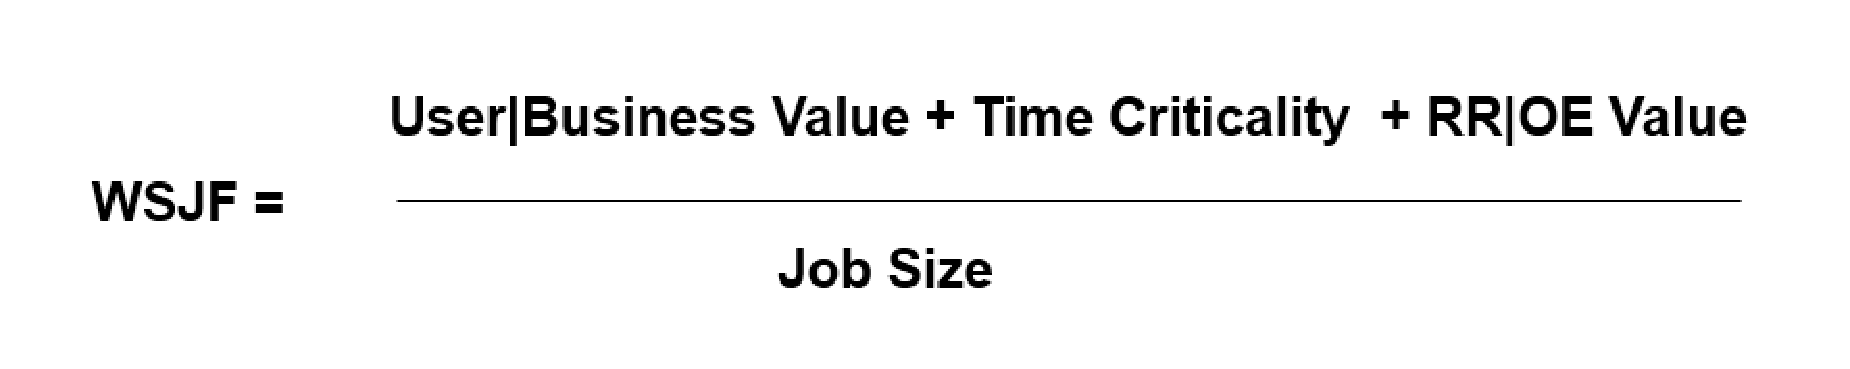
\includegraphics[keepaspectratio=true,scale=0.3]{figuras/WSJF-Formula.eps}
        \caption{Fómula do cálculo do valor de uma feature.}
        \label{fig:wsjf}
    \end{figure}


  \end{description}


  \subsection{Atividades}

  \begin{table}[H]
    \centering
      \begin{tabular}{| m{5em} | m{10cm} |}
        \hline
        ID       & 04   \\ \hline
        Nome     & Levantar Requisitos Não Funcionais   \\ \hline
        Objetivo & Serão realizadas reuniões entre o cliente e o time. Serão levantas as melhores condições para a solução. Ex: Tecnologia, Plataforma, Usabilidade. Também serão levantadas as restrições e padrões que o projeto deve seguir. \\ \hline
        Entradas & \textit{Backlog} do Programa e \textit{Backlog} do portfólio.   \\ \hline
        Saídas   & Visão \\ \hline
        Papel Responsável   & Gerente de Programa. \\ \hline
      \end{tabular}
      \caption{Atividade: Levantar Requisitos Não Funcionais}
      \label{tabela:atividade4}
  \end{table}

  \begin{table}[H]
    \centering
      \begin{tabular}{| m{5em} | m{10cm} |}
        \hline
        ID       & 05   \\ \hline
        Nome     & Selecionar Épico para Iteração   \\ \hline
        Objetivo & Atividade de priorização dos épicos, onde serão selecionados os épicos a serem abordados na iteração de acordo com o \textit{Backlog} do portfólio. \\ \hline
        Entradas & \textit{Backlog} do portfólio.\\ \hline
        Saídas   & Épico da iteração \\ \hline
        Papel Responsável   & Gerente de Programa. \\ \hline
      \end{tabular}
      \caption{Atividade: Selecionar Épico para Iteração}
      \label{tabela:atividade5}
  \end{table}

  \begin{table}[H]
    \centering
      \begin{tabular}{| m{5em} | m{10cm} |}
        \hline
        ID       & 06   \\ \hline
        Nome     & Levantar de \textit{Features}    \\ \hline
        Objetivo & Atividade para levantar detalhadamente as \textit{Features}  que estão relacionadas aos épicos selecionados. \\ \hline
        Entradas & Épico da Iteração\\ \hline
        Saídas   & \textit{Backlog} do Programa \\ \hline
        Papel Responsável   & Gerente de Programa. \\ \hline
      \end{tabular}
      \caption{Atividade: Levantar de \textit{Features} }
      \label{tabela:atividade6}
  \end{table}

  \begin{table}[H]
    \centering
      \begin{tabular}{| m{5em} | m{10cm} |}
        \hline
        ID       & 07   \\ \hline
        Nome     & Levantar Histórias da Release  \\ \hline
        Objetivo & Atividade para levantar histórias de usuários, relacionadas as \textit{Features}  levantadas, em alto nível, sem detalhamentos. Aqui é necessária a aprovação do Gerente para sair da atividade.  \\ \hline
        Entradas & \textit{Backlog} do Programa\\ \hline
        Saídas   & \textit{Backlog} do Time \\ \hline
        Papel Responsável   & Gerente de Programa. \\ \hline
      \end{tabular}
      \caption{Atividade: Levantar Histórias da Release}
      \label{tabela:atividade7}
  \end{table}

  \begin{table}[H]
    \centering
      \begin{tabular}{| m{5em} | m{10cm} |}
        \hline
        ID       & 08   \\ \hline
        Nome     & Planejar Releases  \\ \hline
        Objetivo & Atividade para planejar as releases da iteração, irá gerá o \textit{Roadmap}e o program \textit{Backlog} com as \textit{Features}  priorizadas e organizada em uma linha do tempo de entregas. São definidos os objetivos de cada release. É realizada uma validação com o cliente a é necessária a aprovação do Gerente. Após essa atividade é realizado em paralelo a Gerência de Mudanças. \\ \hline
        Entradas & \textit{Backlog} do Time, \textit{Backlog} do Programa. \\ \hline
        Saídas   & \textit{Backlog} do Programa, \textit{Roadmap}\\ \hline
        Papel Responsável   & Gerente de Programa. \\ \hline
      \end{tabular}
      \caption{Atividade: Planejar Releases}
      \label{tabela:atividade8}
  \end{table}

  \begin{table}[H]
    \centering
      \begin{tabular}{| m{5em} | m{10cm} |}
        \hline
        ID       & 18   \\ \hline
        Nome     & Integrar Módulos de Software  \\ \hline
        Objetivo & Ativida para integração dos módulos de software que foram desenvolvidos. \\ \hline
        Entradas & Módulos de Software. \\ \hline
        Saídas   & Pacote de Software. \\ \hline
        Papel Responsável   & Gerente de Programa. \\ \hline
      \end{tabular}
      \caption{Atividade: Integrar Módulos de Software}
      \label{tabela:atividade18}
  \end{table}

  \begin{table}[H]
    \centering
      \begin{tabular}{| m{5em} | m{10cm} |}
        \hline
        ID       & 19   \\ \hline
        Nome     & Entregar Release  \\ \hline
        Objetivo & Atividade para lançamento de um novo pacote de software, após as integração dos módulos o pacote fica disponível o que representa entrega de valor direto para o cliente. \\ \hline
        Entradas & Pacote de Software. \\ \hline
        Saídas   & -- \\ \hline
        Papel Responsável   & Gerente de Programa. \\ \hline
      \end{tabular}
      \caption{Atividade: Entregar Release}
      \label{tabela:atividade16}
  \end{table}

\section{Time}
  \subsection{Processo}

  \begin{figure}[H]
      \centering
    \includegraphics[keepaspectratio=true,scale=0.5]{figuras/time.eps}
      \caption{Visão geral do nível de time.}
      \label{fig:time}
  \end{figure}

  \subsection{Papéis}

\textbf{Dono do Produto}: Responsável por definir, manter e priorizar o \textit{Backlog} do time,
elaborar e validade as histórias de usuário, participar do planejamento e validação
da Sprint de tal modo a agilizar a execução de programas prioritários, mantendo a
integridade conceitual e técnica dos recursos ou componentes do time. Possui um papel
significativo no que se diz respeito a qualidade.

\textbf{Scrum Master}: Responsável por facilitar as interações da equipe e ajuda
a dirigir os esforços da equipe para a melhora continua.

\textbf{Team}: São os indivíduos capazes de definir, construir e testar em uma interação
de curto tempo. Inclui desenvolvedores, testadores, um Scrum Master e Dono do Produto.

  \subsection{Artefatos}

\begin{description}
  \item[A - \textit{Backlog} do Time]
  Tem como conteúdo, basicamente todas as coisa que o time deve fazer para gerar
  os pacotes de software e entregar valor para o cliente. É composto por histórias
  de usuário, histórias técnicas, defeitos, necessidades de infraestrutura, necessidades
  do time, refatoração, e qualquer outra coisa que o time precisa fazer. Muitas entidades
  contribuem para a geração do \textit{Backlog} do time como representado na imagem abaixo:

  \begin{figure}[H]
      \centering
    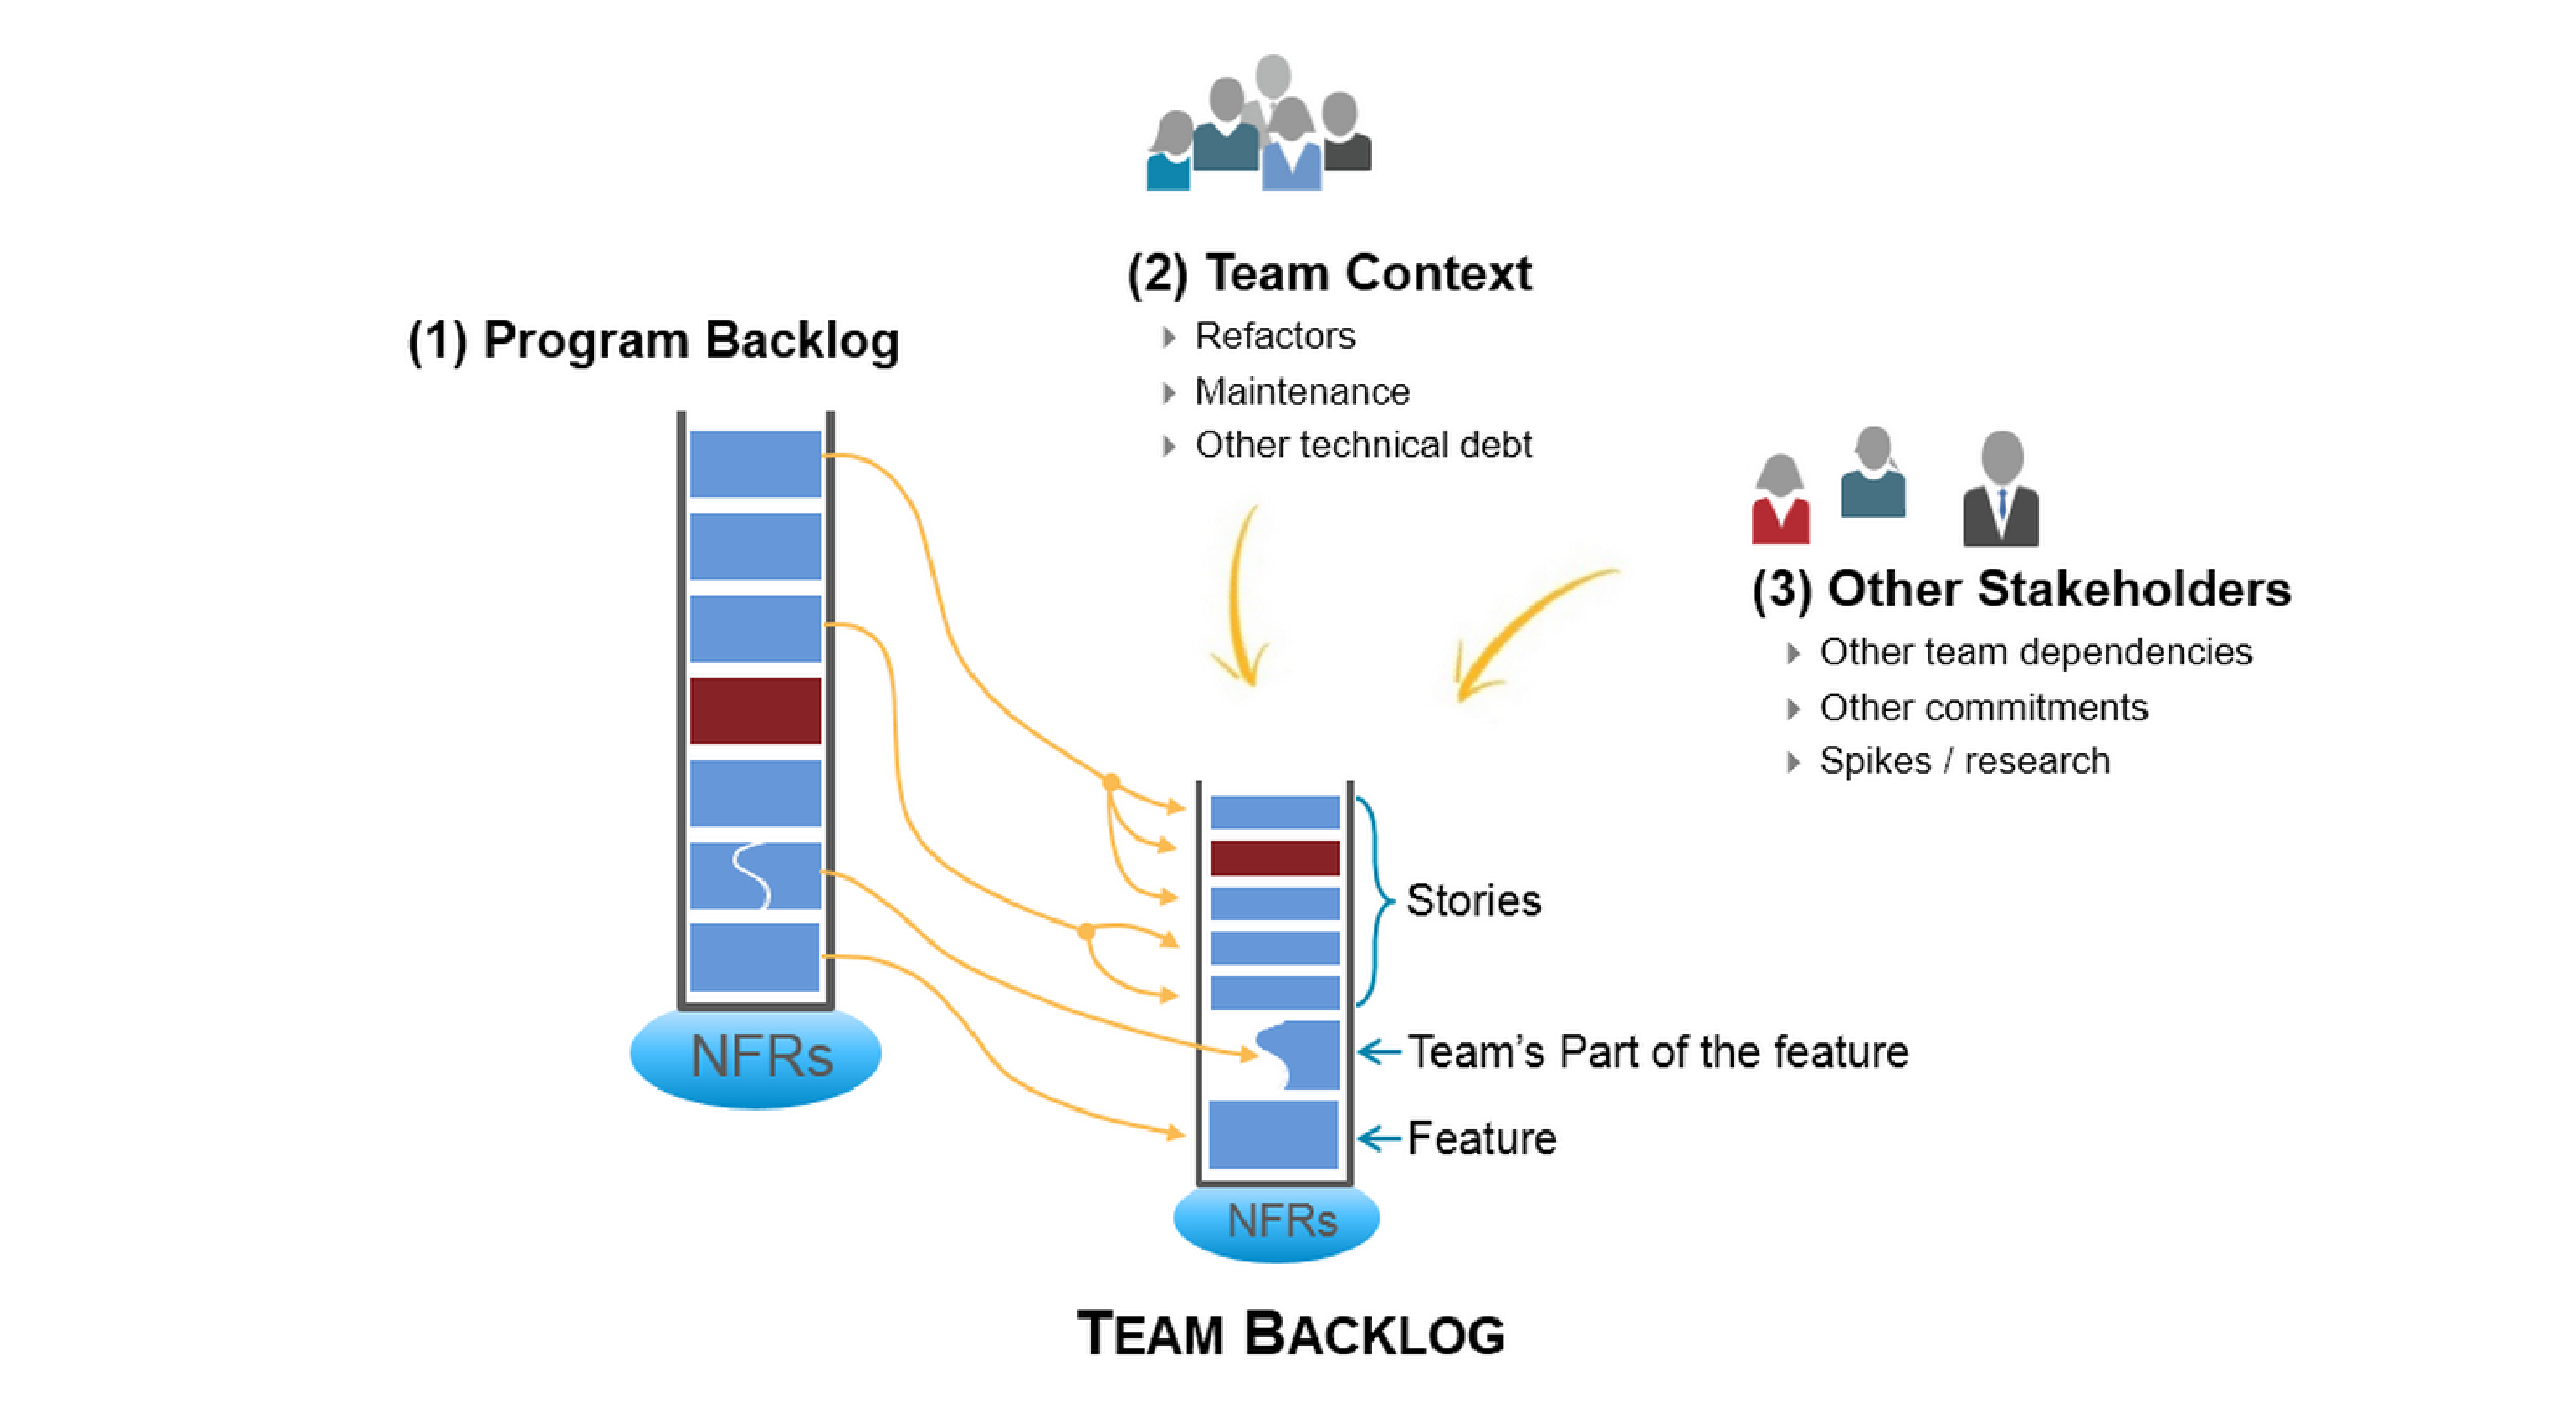
\includegraphics[keepaspectratio=true,scale=0.3]{figuras/TeamBacklog.eps}
      \caption{Estruturação do \textit{Backlog} do time.}
      \label{fig:backlog}
  \end{figure}

  Nota-se que na criação do \textit{Backlog} de time as \textit{Features}  são ramificadas em pequenas histórias.


  \item[B - Lista de melhorias e Correções]
   E gerada para registrar evoluções nos artefatos que foram obtidas através de feedbacks
  de algum artefato já entregue. Presente em vários níveis.

\end{description}


  \subsection{Atividades}

  \begin{table}[H]
    \centering
      \begin{tabular}{| m{5em} | m{10cm} |}
        \hline
        ID       & 09   \\ \hline
        Nome     & Detalhar Histórias de Usuário  \\ \hline
        Objetivo & Serão detalhados as histórias relativas as \textit{Features}  corrente, como principal objetivo definir os critériaos de aceitação para teste das mesmas.  \\ \hline
        Entradas & Roadmap, \textit{Backlog} do Time\\ \hline
        Saídas   & \textit{Backlog} do Time (Refinado) \\ \hline
        Papel Responsável   & Gerente de Produto. \\ \hline
      \end{tabular}
      \caption{Atividade: Detalhar Histórias de Usuário}
      \label{tabela:atividade9}
  \end{table}

  \begin{table}[H]
    \centering
      \begin{tabular}{| m{5em} | m{10cm} |}
        \hline
        ID       & 10   \\ \hline
        Nome     & Levantar e Priorizar Necessidades do Time  \\ \hline
        Objetivo & Serão identificados os spikes, necessidades que o time precisa suprir durante a sprint, para evoluir.  \\ \hline
        Entradas & \textit{Backlog} do Time (Refinado)\\ \hline
        Saídas   & \textit{Backlog} do Time (Refinado) \\ \hline
        Papel Responsável   & Gerente de Produto. \\ \hline
      \end{tabular}
      \caption{Atividade: Levantar e Priorizar Necessidades do Time}
      \label{tabela:atividade10}
  \end{table}

  \begin{table}[H]
    \centering
      \begin{tabular}{| m{5em} | m{10cm} |}
        \hline
        ID       & 11   \\ \hline
        Nome     & Planejar Sprints  \\ \hline
        Objetivo & Serão  organizadas as histórias e tarefas em sprints. É necessária a aprovação do Gerente de produto. Após a atividade é realizada a Gerência de mudança em paralelo.  \\ \hline
        Entradas & \textit{Backlog} do Time (Refinado)\\ \hline
        Saídas   & \textit{Backlog} do Time (Refinado) \\ \hline
        Papel Responsável   & Gerente de Portfólio. \\ \hline
      \end{tabular}
      \caption{Atividade: Planejar Sprints}
      \label{tabela:atividade11}
  \end{table}

  \begin{table}[H]
    \centering
      \begin{tabular}{| m{5em} | m{10cm} |}
        \hline
        ID       & 12   \\ \hline
        Nome     & Desenvolver  Sprint  \\ \hline
        Objetivo & Subprocesso de desenvolvimento da sprint, onde ocorrerá a codificação de testes e histórias, e validação com o usuário.  \\ \hline
        Entradas & \textit{Backlog} do Time (Refinado)\\ \hline
        Saídas   & Módulo de Software. \\ \hline
        Papel Responsável   & Mestre Scrum e Time. \\ \hline
      \end{tabular}
      \caption{Atividade: Desenvolver  Sprint}
      \label{tabela:atividade12}
  \end{table}

  \begin{table}[H]
    \centering
      \begin{tabular}{| m{5em} | m{10cm} |}
        \hline
        ID       & 13   \\ \hline
        Nome     & Retrospectiva da Sprint  \\ \hline
        Objetivo & Aqui serão apresentados os componentes desenvolvidos e caso haja uma próxima iteração, será preparado o ambiente para a mesma. Apos a atividade é realizada a Gerência de Mudanças em Paralelo.  \\ \hline
        Entradas & Módulo de Software. \\ \hline
        Saídas   & \textit{Backlog} do Time(Atualizado). \\ \hline
        Papel Responsável   & Gerente de Produto. \\ \hline
      \end{tabular}
      \caption{Atividade: Retrospectiva da Sprint}
      \label{tabela:atividade13}
  \end{table}

  \subsection{Sub-processo de Desenvolvimento}

  Aqui será aberto o sub-process de Desenvolvimento, para uma demonstração de suas atividades, o sub-processo tem como principal objetivo
  engregar um módulo de software de qualidade, validado com o cliente.

    \begin{figure}[H]
        \centering
      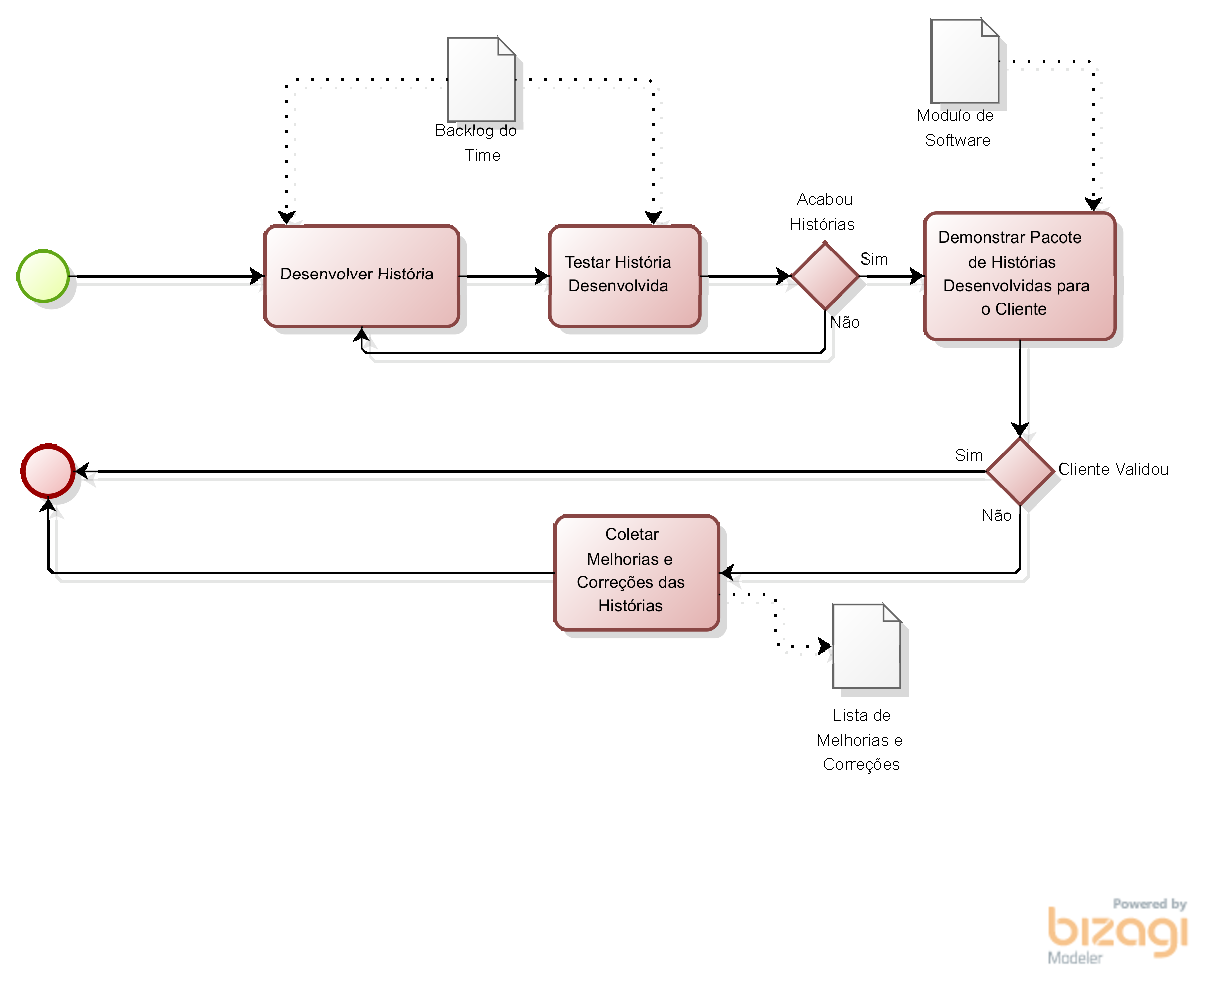
\includegraphics[keepaspectratio=true,scale=0.6]{figuras/desenvolves.eps}
        \caption{Visão geral do sub-processo de desenvolvimento.}
        \label{fig:gerencia}
    \end{figure}


    \begin{table}[H]
      \centering
        \begin{tabular}{| m{5em} | m{10cm} |}
          \hline
          ID       & 14   \\ \hline
          Nome     & Desenvolver Histórias  \\ \hline
          Objetivo & Items do \textit{Backlog} do Time serão desenvolvidos  \\ \hline
          Entradas & \textit{Backlog} do Time (Refinado)\\ \hline
          Saídas   & Candidato a versões de Software \\ \hline
          Papel Responsável   & Time. \\ \hline
        \end{tabular}
        \caption{Atividade: Desenvolver Histórias}
        \label{tabela:atividade14}
    \end{table}

    \begin{table}[H]
      \centering
        \begin{tabular}{| m{5em} | m{10cm} |}
          \hline
          ID       & 15   \\ \hline
          Nome     & Testar Histórias Desenvolvidas  \\ \hline
          Objetivo & Itens do \textit{Backlog} do Time serão testados internamente. Caso não passe no teste, Precisa ser corrigido para sair dessa atividade.  \\ \hline
          Entradas & \textit{Backlog} do Time (Refinado)\\ \hline
          Saídas   & Versão de Software \\ \hline
          Papel Responsável   & Time. \\ \hline
        \end{tabular}
        \caption{Atividade: Testar Histórias Desenvolvidas}
        \label{tabela:atividade15}
    \end{table}

    \begin{table}[H]
      \centering
        \begin{tabular}{| m{5em} | m{10cm} |}
          \hline
          ID       & 16   \\ \hline
          Nome     & Demonstrar Pacote de histórias desenvolvidas para o cliente. \\ \hline
          Objetivo & Pacote de software será demonstrado para o cliente. \\ \hline
          Entradas & Modulo de Software\\ \hline
          Saídas   &  --- \\ \hline
          Papel Responsável   & Mestre Scrum. \\ \hline
        \end{tabular}
        \caption{Atividade: Demonstrar Pacote de histórias desenvolvidas para o cliente.}
        \label{tabela:atividade16}
    \end{table}

    \begin{table}[H]
      \centering
        \begin{tabular}{| m{5em} | m{10cm} |}
          \hline
          ID       & 17   \\ \hline
          Nome     & Coletar Melhorias e correções das histórias  \\ \hline
          Objetivo & Coletar feedbacks do usuário para constante refinamento do sistema.  \\ \hline
          Entradas & ---\\ \hline
          Saídas   & Lista de melhorias e correções. \\ \hline
          Papel Responsável   & Time. \\ \hline
        \end{tabular}
        \caption{Atividade: Coletar Melhorias e correções das histórias}
        \label{tabela:atividade17}
    \end{table}


\section{Gerência de Mudança}\label{sec:gerencia}

  Este sub-processo é responsável por manter a rastreabilidade e concistência dos requisitos.
  Está presente em todos os nível do processo, uma vez que podem haver mudanças que impactam todos
  os níveis. Por exemplo: Suponha que haja uma mudança durante o desenvolvimento de uma sprint.
  Essa mudança deve ser atualizada no \textit{Backlog} do time, caso essa nova história não esteja mapeada com
  uma feature, deve-se atualizar o \textit{Backlog} do programa e o mesmo para o \textit{Backlog} do portfólio.

\subsection{Processo}
  \begin{figure}[H]
      \centering
    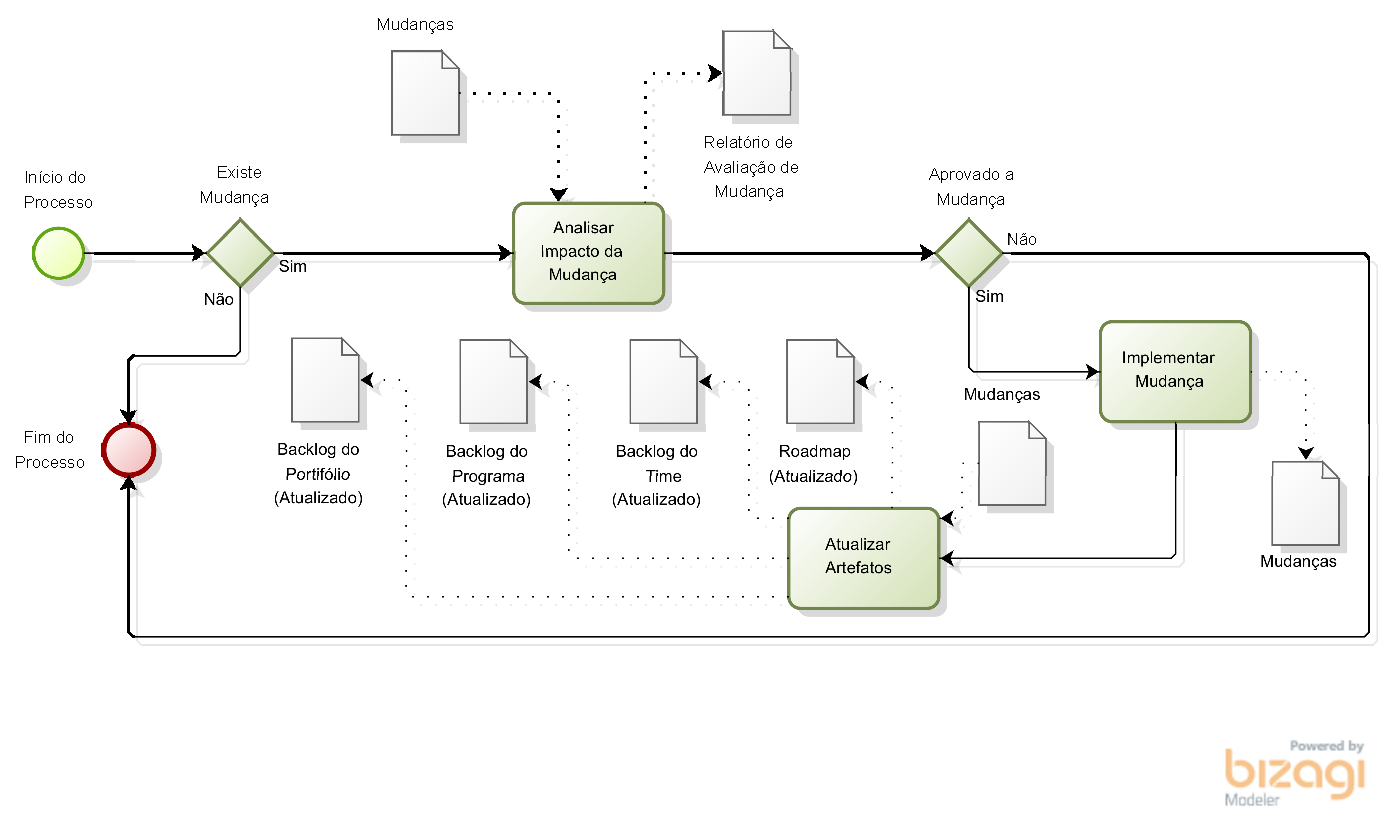
\includegraphics[keepaspectratio=true,scale=0.6]{figuras/gerencia.eps}
      \caption{Visão geral do processo de gerência de mudança.}
      \label{fig:gerencia}
  \end{figure}

\subsection{Papéis}

  \textbf{GERENTE DE PORTFÓLIO}: No tratamento de mudanças, não haverá um papel especifico devido
à dimensão do projeto, cabendo a ele a responsabilidade de também gerir mudanças, caso necessário.

\subsection{Artefatos}

\begin{description}
  \item[A - Solicitação de Mudança: ]
  Lista com as mudanças que necessitam ser analisadas pela gerência, a lista contém
  uma síntese detalhando porque a mudança foi solicitada.
  \item [B - Mudanças: ] Representa a rastreabilidade dessa mudança, detalhando em
  quais níveis ela irá impactar e qual será o custo para efetivar essa mudança.
  \item [C - Relatório de Avaliação de mundanças: ] O relatório explica o motivo e impactos da aceite
  ou recusa de uma mudança, e serve como base para realização das mudanças.
\end{description}

\subsection{Atividades}

\begin{table}[H]
  \centering
    \begin{tabular}{| m{5em} | m{10cm} |}
      \hline
      ID       & 20   \\ \hline
      Nome     & Analisar Impacto da Mudança \\ \hline
      Objetivo & Caso haja mudança nos requisitos do sistema, a atividade será acionada para rastrear, analisar qual o impacto e viabilidade para aprovação ou recusa da mudança.  \\ \hline
      Entradas & Mudanças \\ \hline
      Saídas   & Relatório de Avaliação de Mudança \\ \hline
      Papel Responsável   & Gerente de Portfólio. \\ \hline
    \end{tabular}
    \caption{Atividade: Analisar Impacto da Mudança}
    \label{tabela:atividade20}
\end{table}

\begin{table}[H]
  \centering
    \begin{tabular}{| m{5em} | m{10cm} |}
      \hline
      ID       & 21   \\ \hline
      Nome     & Implementar Mudança \\ \hline
      Objetivo & Executa ações necessárias para implementar a mudança aprovada.  \\ \hline
      Entradas & Mudanças \\ \hline
      Saídas   & -- \\ \hline
      Papel Responsável   & Gerente de Portfólio. \\ \hline
    \end{tabular}
    \caption{Atividade: Implementar Mudança}
    \label{tabela:atividade21}
\end{table}

\begin{table}[H]
  \centering
    \begin{tabular}{| m{5em} | m{10cm} |}
      \hline
      ID       & 22   \\ \hline
      Nome     & Atualizar Artefatos  \\ \hline
      Objetivo & Após Implementada a mudança, a documentação tem que ser atualizada para garantir a rastreabilidade e consistência dos requisitos.  \\ \hline
      Entradas & Mudanças\\ \hline
      Saídas   & Artefatos Atualizados  \\ \hline
      Papel Responsável   & Gerente de Portfólio. \\ \hline
    \end{tabular}
    \caption{Atividade: Atualizar Artefatos}
    \label{tabela:atividade22}
\end{table}
